% !TeX root = main.tex

\chapter{Sparse Matrix Vector Multiplication}
\glsresetall
\label{chapter:spmv}

Sparse matrix vector multiplication (SpMV) takes a sparse matrix, i.e., one in which most of its elements  are zero, and multiplies it by a vector. The vector itself may be sparse as well, but often it is dense. This is a common operation in scientific applications, economic modeling, data mining, and information retrieval. For example, it is used as an iterative method for solving sparse linear systems and eigenvalue problems. It is an operation in PageRank and it is also used in computer vision, e.g., image reconstruction.

This chapter introduces several new HLS concepts, and reinforces some previously discussed optimization. One goal of the chapter is to introduce a more complex data structure. We use a \gls{crs} representation to hold the sparse matrix. Another goal is to show how to perform testing. We build a simple structure for a testbench that can be used to help determine if the code is functionally correct. This is an important aspect of hardware design, and \VHLS makes it easy to test many aspects of the generated RTL with the same high-level C testbench. This is one of the big advantages of HLS over RTL design. We also show how you can perform C/RTL cosimulation using the testbench and \VHLS tool. This is necessary to derive the performance characteristics for the different SpMV designs. Since the execution time depends upon the number of entries in the sparse matrix, we must use input data in order to determine the clock cycles for the task interval and task latency.

\section{Background}

\begin{figure}
\centering
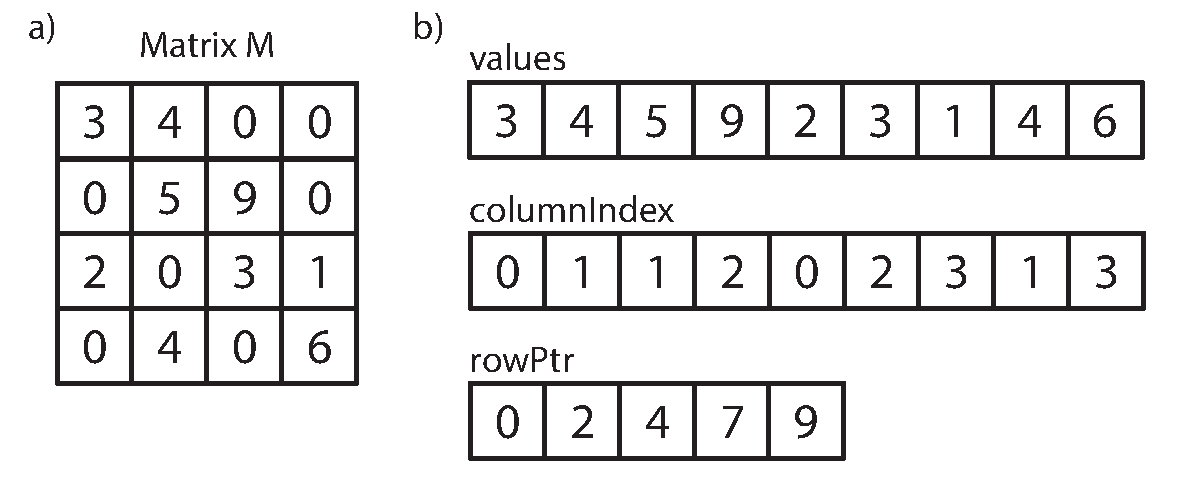
\includegraphics[width=  .65\textwidth]{images/crs}
\caption{A $4 \times 4$ matrix $\mathbf{M}$ represented in two different ways: as a `dense' matrix stored in a two-dimensional array, and as a sparse matrix stored in the compressed row storage (\gls{crs}) form, a data structure consisting of three arrays. }
\label{fig:crs}
\end{figure}

Figure~\ref{fig:crs} shows an example of a $4 \times 4$ matrix $\mathbf{M}$ represented in two different ways.  Figure ~\ref{fig:crs} a) shows the normal representation of the matrix as a two-dimensional array of 16 elements.  Each element is store in its own location in the array.  Figure ~\ref{fig:crs} b) shows the same matrix represented in \gls{crs} format.   The \gls{crs} representation is a data structure consisting of three arrays.  The \lstinline{values} array holds the value of each non-zero element in the matrix. The \lstinline{columnIndex} and \lstinline{rowPtr} arrays encode information about the location of these non-zero elements in the matrix. \lstinline{columnIndex} stores the column of each element, while \lstinline{rowPtr} contains the index in \lstinline|values| of the first element in each row. The \gls{crs} format avoids storing values in the matrix that are zero, although there is nothing to prevent a zero from being explicitly represented in the \lstinline|values| array.  In the example, however, we see that the \lstinline|values| array does not, in fact, contain any zero elements.  The tradeoff is that some additional book-keeping information (the \lstinline|columnIndex| and \lstinline|rowPtr| arrays) in order to properly interpret and manipulate the matrix.  The \gls{crs} form is commonly used when large matrices contain only a small number of non-zero elements (typically 10 percent or less), enabling these matrices to be stored with less memory and manipulated with fewer operations. However, the \gls{crs} form has no requirements about the sparsity of the matrix and can be used for any matrix. This makes it a general approach that can be used for any matrix, but not necessarily the most efficient.  The \gls{crs} form is also not the only efficient representation of sparse matrices.  Depending on the characteristics of the matrix and the types of operations to be performed, other sparse representations can also be used.

More precisely, the \gls{crs} format uses a data structure consisting of three arrays: \lstinline{values}, \lstinline{colIndex}, and \lstinline{rowPtr}. The \lstinline{values} array and the \lstinline{columnIndex} has an entry for each of the non-zero elements in the sparse matrix $\mathbf{M}$. These arrays represent the matrix $\mathbf{M}$ stored in a row-wise fashion, i.e., left to right, and top to bottom. The data in the matrix is stored in the \lstinline|values| array, while the \lstinline{columnIndex} array contains the horizontal location of the data in the matrix.  If \lstinline|values[k]| represents $M_{ij}$ then \lstinline|colIndex[k]| = j. The array \lstinline{rowPtr} has size $n+1$ for an $n$-row matrix.  \lstinline|rowPtr[k]| contains the total number of elements in all the rows in the matrix prior to row $k$, with the first element \lstinline|rowPtr[0] = 0| and the last element \lstinline|rowPtr[n]| always giving the total number of non-zero elements the matrix.  As a result, if \lstinline|values[k]| represents $M_{ij}$, then \lstinline|rowPtr[i]| $\leq k < $\lstinline|rowPtr[i+1]|.  If row \lstinline|k| contains any non-zero elements, then \lstinline|rowPtr[k]| will contain the index of the first element in the row.  Note that if there are rows in the matrix without a non-zero element, then values in the \lstinline|rowPtr| array will repeat.

Looking at Figure~\ref{fig:crs} a), we can scan the matrix in row-major order to determine the \lstinline{values} array in \gls{crs} form.  Whenever we find a non-zero element, its value is stored at the next available index $i$ in the \lstinline|values| array and its column is stored at \lstinline{columnIndex[i]}.  In addition, whenever we start scanning a new row, we store the next available index $i$ in the \lstinline|rowPtr| array.  As a result, the first element in the \lstinline|rowPtr| array is always zero. 
Looking at Figure~\ref{fig:crs} b), we can also convert the matrix back to a two-dimensional array representation.  The first step is to determine the number of elements in each row of the matrix from the \lstinline|rowPtr| array.  The number of elements in row $i$ is the difference \lstinline|rowPtr[i]-rowPtr[i+1]|.   Then the row can be reconstructed by iterating through the \lstinline|values| array starting at \lstinline|values[rowPtr[i]]|. In our example matrix, the because the first two elements of the \lstinline|rowPtr| array are $0$ and $2$, then we know that there are 2 elements in the first row, i.e., \lstinline|values[0]| and \lstinline|values[1]|.  The first non-zero element in the \lstinline{values} data structure, \lstinline|values[0]|, is $3$.  This value is in column 0, since \lstinline{columnIndex[0]} = 0. Similarly, the second non-zero value is the value 4 in column 1. The second row of the matrix has elements with $k \in [2,4)$,  the third row has elements with $k \in [4,7)$, and so on.  In this case, there are 9 non-zero entries, thus that last entry in the \lstinline{rowPtr} data structure is 9. 
 
\begin{exercise}
Given a 2-dimensional array representing a matrix, write the C code to convert the matrix to \gls{crs} form.  Write the corresponding C code to convert the matrix in \gls{crs} form back to a 2-dimensional array.
\end{exercise}

It turns out that using the \gls{crs} form, we can multiply a sparse matrix with a vector relatively efficiently without explicitly converting the matrix back to a 2-dimensional array.  In fact, for large matrices with a small number of non-zero elements, sparse matrix-vector multiply is much more efficient than the dense matrix-vector multiply we discussed in chapter \ref{chapter:dft}.  This is because we can compute the non-zero elements of the result by only looking at the non-zero elements of the operands. 

\section{Baseline Implementation}

\begin{figure}
\lstinputlisting{examples/spmv.cpp}
\caption{  The baseline code for sparse matrix vector (SpMV) multiplication, which performs the operation $y = \mathbf{M} \cdot x$. The variables \lstinline{rowPtr}, \lstinline{columnIndex}, and \lstinline{values}  hold $\mathbf{M}$ in \gls{crs} format. The first \lstinline{for} loop iterates across the rows while the second nested \lstinline{for} loop iterates across the columns of $\mathbf{M}$ by multiplying each non-zero element by the corresponding element in the vector \lstinline{x} which results in one element in the resulting vector \lstinline{y}. }
\label{fig:spmv_arch1}
\end{figure}

\begin{figure}
\lstinputlisting{examples/spmv.h}
\caption{ The header file for \lstinline{spmv} function and testbench.  }
\label{fig:spmv.h}
\end{figure}

Figure \ref{fig:spmv_arch1} provides a baseline code for sparse matrix vector multiplication. The \lstinline{spmv} function has five arguments. The arguments \lstinline{rowPtr}, \lstinline{columnIndex}, and \lstinline{values} correspond to the input matrix $\mathbf{M}$ in \gls{crs} format. These are equivalent to the data structures shown in Figure \ref{fig:crs}. The argument \lstinline{y} holds the output result $y$ and the argument \lstinline{x} holds the input vector $x$ to be multiplied by the matrix.  The variable \lstinline{NUM_ROWS} indicates the number of rows in the matrix $\mathbf{M}$. The variable \lstinline{NNZ} is the number of non-zero elements in the matrix $\mathbf{M}$. Finally, the variable \lstinline{SIZE} is the number of elements in the arrays \lstinline{x} and \lstinline{y}.

The outer \lstinline{for} loop, labeled \lstinline{L1}, iterates across each row of the matrix. Multiplying this row of the matrix with the vector $x$ will produce one element of $y$.  The inner loop labeled \lstinline{L2} loop across the elements in the columns of the matrix $\mathbf{M}$. The \lstinline{L2} loop iterates \lstinline{rowPtr[i+1]} $-$ \lstinline{rowPtr[i]} times, corresponding to the number of non-zero entries in that row. For each entry, we read the value of the non-zero element of the $\mathbf{M}$ matrix from the \lstinline{values} array and multiply it by the corresponding value of the vector $x$ read from the \lstinline{x} array. That value is located at \lstinline{columnIndex[k]} since the data structure \lstinline{columnIndex} holds the column for the value \lstinline{k}. 

\begin{figure}
\lstinputlisting[format=none]{examples/spmv-top.cpp}
\caption{  A simple testbench for our \lstinline{spmv} function. The testbench generates one example and computes the matrix vector multiplication using a sparse (\lstinline{spmv}) and non-sparse function (\lstinline{matrixvector}).}
\label{fig:spmv_test}
\end{figure}

\section{Testbench}

Figure \ref{fig:spmv_test} shows a simple testbench for the \lstinline{spmv} function. The testbench starts by defining the \lstinline{matrixvector} function. This is a straightforward implementation of matrix vector multiplication. This does not assume a sparse matrix and does not use the \gls{crs} format. We will compare the output results from this function with the results from our \lstinline{spmv} function. 

\begin{aside}
A common testbench will implement a ``golden'' reference implementation of the function that the designer wishes to synthesis. The testbench will then compare the results of the golden reference with those generated from the code that is synthesized by the \VHLS code. A best practice for the testbench is to use alternative implementations for the golden reference and the synthesizable code. This provides more assurance that both implementations are correct. 
\end{aside}

The testbench continues in the \lstinline{main} function. Here we set the \lstinline{fail} variable equal to $0$ (later code sets this to $1$ if the output data from \lstinline{spmv} does not match that from the function \lstinline{matrixvector}). Then we define a set of variables that correspond to the matrix $\mathbf{M}$, the input vector $x$ and the output vector $y$. In case of $\mathbf{M}$, we have both the ``normal'' form and the CSR form (stored in the variables \lstinline{values}, \lstinline{columnIndex}, and \lstinline{rowPtr}). The values of the $\mathbf{M}$ matrix are the same as shown in Figure \ref{fig:crs}. We have two versions of the output vector $y$. The \lstinline{y_sw} array stores the output from the function \lstinline{matrixvector} and the \lstinline{y} array has the output from the function \lstinline{spmv}. 

After defining all of the input and output variables, we call the \lstinline{spmv} and \lstinline{matrixvector} functions using the appropriate data. The following \lstinline{for} loop compares the output results from both of the functions by comparing the elements from \lstinline{y_sw} with those in \lstinline{y}. If any of them are different, we set the \lstinline{fail} flag equal to $1$. Lastly, we print out the results of the test and then return the \lstinline{fail} variable. 

This testbench is relatively simple and probably insufficient to ensure that the implementation is correct.  Primarily, it only tests one example matrix, whereas a better testbench would test multiple matrices.  It is common, for instance, to randomly generate inputs for testing, in addition to explicitly verifying important corner-cases.   In this case, we need to make sure to vary not only the values being operated on, which which will be passed to our accelerator when it is executing, but also to vary the compile-time parameters which might be used to create different accelerators with different tradeoffs.  The key difference is that we can randomly generate multiple data values to operate on and test them all in the same execution of the program, using multiple function calls.   Compile-time parameters, on the other hand, require the code to be recompiled every time parameters change.

\begin{exercise}
Create a more sophisticated testbench which generates multiple sets of test data using a random number generator. The compile-time parameters of the sparse matrix should be modifiable (e.g., \lstinline{SIZE}, \lstinline{NNZ}, etc.).  Create an HLS synthesis script which executes the same code multiple times for different reasonable compile-time parameters.
\end{exercise}

\section{Specifying Loop Properties}

If you directly synthesize this code, you will get results for the clock period and utilization. However, you will not get the number of clock cycles either in terms of task latency or initiation interval. This is because this depends upon the input data, which is external to the \lstinline{spmv} function itself.  Primarily, the performance depends on the number of times the body of the inner loop is executed, which is equal to the number of non-zero elements in $\mathbf{M}$.  We know that the number of non-zero elements is limited by the constant \lstinline{NNZ} in the code, but it is possible to call the code with matrices of different sizes, so the actual number of iterations is data-dependent. In addition, the performance may vary depending on the location of the non-zero elements and the optimization directives utilized during synthesis. To make matters worse, the number of iterations depends on the input in a complex way and many potential inputs don't actually represent valid matrices. Thus, it is very difficult for a tool to determine the total number of clock cycles for the \lstinline{spmv} function without complex analysis and additional information. \VHLS is unable to perform this analysis.

\begin{exercise}
What are the preconditions for the spmv function to work correctly?  Prove that given these preconditions, the body of the inner loop does, in fact, execute exactly once for each non-zero element in the matrix.
\end{exercise}

There are several ways to leverage the tool to derive some performance estimates, however. One method is to provide the \VHLS tool additional information about the loop bounds. This can be done using the \lstinline{loop_tripcount} directive, which enables the designer to specify a minimum, maximum, and/or average number of iterations for each particular loop. By providing these values, the \VHLS tool is capable of providing an estimate on the number of clock cycles. 

\begin{aside}
Use the \lstinline{loop_tripcount} directive to specify minimum, maximum, and/or average number of iterations for a loop with a variable bound. This enables the \VHLS tool to provide an estimate on the number of clock cycles for the design. This does not impact the results of the synthesis; it only effects the synthesis report.
\end{aside}

\begin{exercise}
Add a \lstinline{loop_tripcount} directive to the \lstinline{spmv} function. The syntax for the pragma form of the directive is \lstinline{#pragma HLS loop_tripcount min=X, max=Y, avg=Z} where \lstinline{X}, \lstinline{Y}, and \lstinline{Z} are constant positive integers. Which loops require this directive? What happens to the synthesis report when you change the different parameters (\lstinline{min}, \lstinline{max}, and \lstinline{avg})? How does this effect the clock period? How does it change the utilization results?
\end{exercise}

The \lstinline{loop_tripcount} directive enables the designer to get a rough idea about the performance of a function. This can enable comparison between different implementations of the same function either by applying different optimization directives or by restructuring the code itself.  However, it may be difficult or impossible to determine the \lstinline{min}, \lstinline{max}, and \lstinline{avg} parameters.  It can also be difficult to provide tight bounds on the \lstinline{min} and \lstinline{max} parameters. If there is a testbench, there is another more accurate method to calculate the total number of clock cycles required for the \lstinline{spmv} function. This is done by performing C/RTL cosimulation. 

\section{C/RTL Cosimulation}

C/RTL cosimulation performs automatic testing of the \gls{rtl} designs that are generated by the \VHLS tool. It does this by executing the synthesized code together with the provided testbench. The execution is instrumented to record the input and output values for each execution of the synthesized code. The input values are converted to cycle-by-cycle \term{input vectors}.  The input vectors are used in an RTL-level simulation of the generated RTL design and the resulting \term{output vectors} are captured.  The testbench code can then be executed again replacing the synthesized code with the captured input and output values.  The testbench code can then return a zero value (indicating success) or a non-zero value (indicating failure).

The C/RTL cosimulation flow combines the cycle-accurate RTL design generated from the \VHLS tool with input values provided from the C testbench. As a result, it can generate accurate estimates of the performance of the generated RTL design which reflect any HLS optimizations, even in the presence of data-dependent behavior.  The minimum, maximum, and average latency and interval of the synthesized function are automatically extracted after simulation completes.

Note that these numbers only correspond to the clock cycles derived from the input data used by the testbench. Thus, they are only as good as the testbench itself. To put it another way, if the testbench does not exercise the function in a manner that is consistent with how it will be used upon deployment, the results will not be accurate. In addition, the input testvectors are generated with idealized timing that does not accurately model the behavior of external interfaces.  The actual performance may be lower if execution stalls waiting for input data, or if there is contention waiting for external memory access to complete.  Nevertheless, it provides a convenient method for determining clock cycles that does not require the designer to estimate the loop bounds for a variable loop.

\begin{aside}
C/RTL cosimulation provides the latency for functions with variable loop bounds. It reports the minimum, maximum, and average clock cycles for function latency and function interval. These latency values are directly dependent upon the input data from the C testbench. 
\end{aside}

\begin{exercise}
What are the minimum, maximum, and average clock cycles for the \lstinline{spmv} function latency and function interval when using the testbench provided in Figure \ref{fig:spmv_test}?
\end{exercise}


\section{Loop Optimizations and Array Partitioning}

Now that we have a method to gather all of the performance and utilization estimates from the \VHLS tool, let us consider how to best optimize the function. Pipelining, loop unrolling, and data partitioning are the most common first approaches in optimizing a design. And the typical approach is to start with the innermost loop, and then move outwards as necessary.

In this example, pipelining the inner \lstinline{L2} loop is perhaps the first and easiest optimization to consider. This overlaps the execution of the consecutive iterations of this loop, which can result is a faster overall implementation. Without pipelining, each iteration of the \lstinline{L2} loop occurs sequentially. Note that the iterations of the \lstinline{L1} loop are still done sequentially. 

\begin{figure}
\centering
%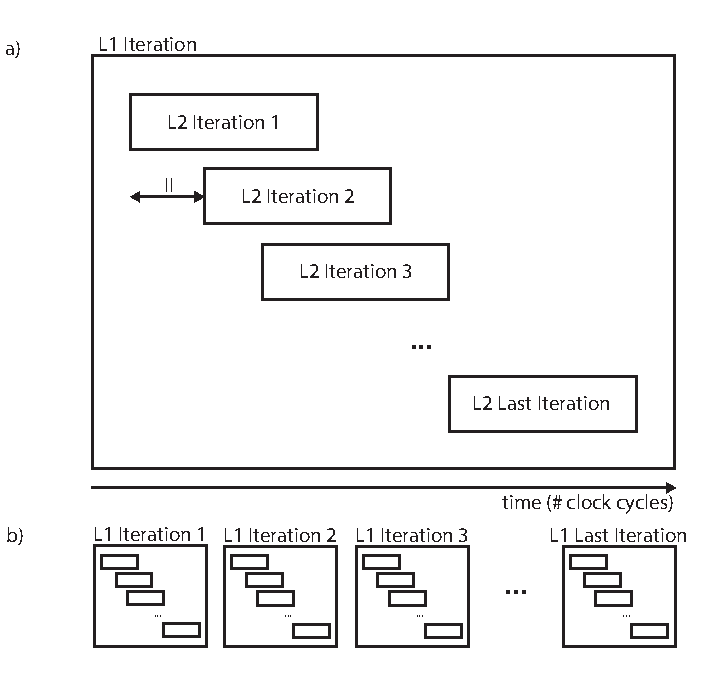
\includegraphics[width=  .85\textwidth]{images/spmv_pipeline_inner}
\includesvg{spmv_behavior}
\caption{Architecture and behavior of the \lstinline{spmv} code with a pipelined inner loop.}
\label{fig:spmv_pipeline_inner}
\end{figure}

Figure \ref{fig:spmv_pipeline_inner} illustrates the approximate manner in which the \lstinline{spmv} function executes when pipelining the \lstinline{L2 for} loop. Each iteration of the inner \lstinline{L2} loop is pipelined with II=3.  Pipelining allows multiple iterations of the inner loop from the same iteration of the outer loop execute concurrently.  In this case, the II of the inner loop is limited by a recurrence through the accumulation.  II=3 is achieved because we've assumed that the adder has a latency of 3 clock cycles.  Iterations of the outer loop are not pipelined, so the inner loop must completely finish and flush the pipeline before the next iteration of the outer \lstinline{L2} loop begins.

\begin{exercise}
Pipeline the innermost \lstinline{L2 for} loop. This can be done by adding a pipeline directive to the \lstinline{spmv} code from Figure \ref{fig:spmv_arch1}. What is the achieved initiation interval (II)? What happens to the results as you specify an II argument, and increase or decrease the target II? 
\end{exercise}

Looking at this behavior, we see that there are several factors limiting the performance of the loop.  One factor is the recurrence through the adder that limits the achieved loop II.  A second factor is that iterations of the outer loop are not pipelined.  An efficient solution for sparse matrix-vector multiply would likely come close to using each multiplier and adder every clock cycle.  This design is far from that.

In Section \ref{subsec:mvmul_implementation} we explored several design optimization techniques, including pipelining different loops, loop unrolling, and array partitioning.  Understanding the tradeoffs between these techniques can be somewhat challenging, since they are often dependent on what another.  We must often apply these techniques together with a carefully chosen goal in mind in order to get a benefit and applying one technique without applying another technique can actually make matters worse.  For instance, when performing loop unrolling, the designer must be careful to understand the effects that this has upon memory accesses. Increasing the number of operations that can execute concurrently doesn't help if performance is limited by available memory ports.  Similarly, providing more memory ports if there are insufficient operations to utilize those memory ports (or if the addresses of each memory operation can't be easily partitioned) can also incur a resource cost without increasing performance.   

% NOTE: most of the description below is redundant with previous discussion and doesn't actually lead to a better design in this case.
%In the \lstinline{spmv} function, we read from three arrays on every iteration of the \lstinline{L2 for} loop -- \lstinline{values}, \lstinline{x}, and \lstinline{columnIndex}. Thus, when we unroll this loop, we need to consider the additional read operations that occur upon these arrays.  Each iteration of the \lstinline{L2 for} loop, accesses \lstinline{values} and \lstinline{columnIndex} using the variable \lstinline{k}, which increases by $1$ on every iteration. In fact, we know that we are accessing these arrays sequentially across the entire function, i.e., last iteration of \lstinline{L2} and the first iteration of the following execution of \lstinline{L2} (as we move to the next iteration of \lstinline{L1}) are sequential. The access pattern of the \lstinline{x} array is a bit more complicated and depends upon the locations of the non-zero elements in the input matrix $\mathbf{M}$. This makes it difficult to optimize these memory accesses. Therefore, we only consider the optimization of the arrays \lstinline{values} and \lstinline{columnIndex}.

%Assume that all of the data in the array \lstinline{values} is stored in one memory. Also assume that the entire array \lstinline{columnIndex} is stored in memory, which is separate from the memory storing \lstinline{values}. Finally, assume that we unroll the \lstinline{L2 for} loop by a factor of four. In this case, each iteration of the unrolled loop requires four read operations from both memories. If the memories do not have four read ports, then the \VHLS tool must sequentialize these read operations. This will reduce the performance. And we are not able to take advantage of all of the parallelism that is exposed by the unroll optimization. 

%We can eliminate the need for sequentialization by creating more read ports. The way to do this is through data partitioning, i.e., separate the \lstinline{values} and \lstinline{columnIndex} into multiple memories. This can be done manually by refactoring the code. Or it can be done automatically by the \VHLS tool using the \lstinline{array_partition} directive. This directive splits the array into multiple smaller memories based upon the \lstinline{factor} argument. For example, setting \lstinline{factor = 2} splits the array into two memories, and \lstinline{factor = 4} divides the array across four memories. 

%The next question is how exactly to divide the arrays. This can be done in a \lstinline{block}, \lstinline{cyclic}, or \lstinline{complete} manner. This is specified using the \lstinline{type} argument. A \lstinline{block} partition takes consecutive elements of the array and puts them in the same memory. For example, the directive \lstinline{#pragma HLS array_partition variable=values block factor=2} will put the elements of the first half of the array \lstinline{values} into one memory and the elements of the second half into another memory. A \lstinline{cyclic} partition takes consecutive elements and puts them in different arrays. Thus, the directive \lstinline{#pragma HLS array_partition variable=values block factor=2} puts every even element of \lstinline{values} into one memory, and every odd element into another separate memory.

%Given that we are accessing the elements from the arrays \lstinline{values} and \lstinline{columnIndex} in a sequential manner, we want to make sure that each consecutive element is in a separate memory. This would be done using a \lstinline{cyclic} partitioning. It should be clear that it is important to consider the data partitioning when we perform loop unrolling.

%Loop unrolling can be used in combination with pipelining. Unrolling reduces the number of iterations of the loop while performing more work per iteration. The addition of pipelining enables the iterations to occur in an overlapping fashion. 

%It is also possible to perform pipelining, unrolling, and data partitioning in combination. However, the effects of each of these is not necessarily straightforward.

To see some of the complexity in applying these combinations of transforms, we encourage you to perform the following exercise:

\begin{exercise}
Synthesize the \lstinline{spmv} design using the directives specified in each of the ten cases from Table \ref{table:spmv_optimizations}. Each case has different pipeline, unroll, and partitioning directives for the different loops and arrays. These partitionings should be done across the three arrays (\lstinline{values}, \lstinline{columnIndex}, and \lstinline{x}). What sort of trends do you see? Does increasing the unroll and partitioning factors help or hurt when it comes to utilization? How about performance? Why?
\end{exercise}

\begin{table}[htbp]
  \centering
  \caption{Potential optimizations for sparse matrix-vector multiplication. }
	\begin{tabular}{*{4}{l}}
    \toprule
    %& \multicolumn{2}{c}{Optimizations}  \\
      %& \multicolumn{2}{c}{Full} & \multicolumn{2}{c}{Full} \\
    %\cmidrule(lr){2-3}
    %\cmidrule(lr){4-6}
    %\cmidrule(lr){8-9}
    %\cmidrule(lr){10-11}
						& L1 		& 		L2 							 \\
    \midrule
    Case 1 & - 			& -  	 \\ 
    Case 2 & - 			& pipeline 	\\ 
    Case 3 & pipeline & - \\
    Case 4 & unroll=2 & - \\ 
    Case 5 & - 			& pipeline, unroll=2 	\\
    Case 6 & - 			& pipeline, unroll=2, cyclic=2 	\\ 
    Case 7 & - 			& pipeline, unroll=4		\\ 
    Case 8 & - 			& pipeline, unroll=4, cyclic=4   \\ 
    Case 9 & - 			& pipeline, unroll=8		\\ 
    Case 10 & - 			& pipeline, unroll=8, cyclic=8   \\ 
    Case 11 & - 			& pipeline, unroll=8, block=8   \\ 
    \bottomrule
  \end{tabular}
  \label{table:spmv_optimizations}
\end{table}

If you performed the previous exercise, you should have seen that blindly applying optimization directives may not always provide you with the expected results. It is usually more effective to consider the properties of an application under design, and to select optimizations with a particular design goal in mind. Of course, this requires some intuition behind the capabilities and limitations of a particular tool being used.  While it is certainly difficult (perhaps impossible?) to understand every detail of a complex tool like \VHLS, we can build a mental model of the most critical aspects.

One of the options we considered in cases 3 and 4 above was to increase pipeline outer loops, such as the \lstinline{L1} loop in this code, rather than inner loops.  This transformation has the effect of increasing the potential parallelism within one task.  In order to perform this optimization, the \VHLS tool must fully unroll inner loops, like the \lstinline{L2} loop in this code. If full unrolling is possible, this can reduce the cost of calculating the loop bounds and can also eliminate recurrences in the code.  However, in this code, the inner loop cannot be unrolled by \VHLS because the loop bound is not constant.

\begin{exercise}
Add a directive to pipeline the outermost \lstinline{L1} loop, i.e., implement case 3 above. What is the initiation interval (II) when you do not set a target II? What happens to the utilization? How does explicitly increasing the II change the utilization results? How does this compare to pipelining the \lstinline{L2} loop? How does this compare to the baseline design (no directives)? What is happening when you attempt to pipeline this outer loop? (hint: check the synthesis log)
\end{exercise}

Another option to increase parallelism is \gls{partial_loop_unrolling} of the inner loop, as in cases 5 through 10.  This transformation exposes more parallelism by allowing more operations from the same loop iteration to be executed concurrently.   In some cases, more operations can increase performance by enabling \VHLS to instantiate more operators when pipelining the inner loop.  However, in this case it is still difficult to improve the II of the inner loop because of the recurrence through the inner loop.  However, in this case, because we have an II greater than 1, many of those operations can be shared on the same operators. 

An partially unrolled version of the code is shown in Figure \ref{fig:spmv_unrolled}.  In this code, the L2 loop has been split into two loops labeled \lstinline|L2_1| and \lstinline|L2_2|.  The innermost \lstinline|L2_2| executes a parameterized number of times, given by the compile-time parameter \lstinline|S|.  The body of the inner loop contains the body of the original \lstinline|L2| loop, along with a condition that arises from the loop bound of the original \lstinline|L2| loop.  In this code, we now have an arbitrary number of multiply and add operations to execute in the body of the \lstinline|L2_1| loop, given by the parameter \lstinline|S|, and a single recurrence through the accumulation \lstinline|y0 += yt|.

Note that the code in Figure \ref{fig:spmv_unrolled} is slightly different from the code that is generated from automatic loop unrolling.  Automatic loop unrolling duplicates operations, but must also preserve the order of each operation (additions in this case).  This results in a long chain of operation dependencies in the inner loop shown on the left side of Figure \ref{fig:spmv_partial_unroll}.  Reordering the operations results in operation dependencies show on the right side of the figure.  In this case, only the final accumulation results in a recurrence.   When using floating-point data types, this reordering of operations can slightly change the behavior of the program, so \VHLS does not apply this kind of operation reordering automatically.  

\begin{figure}
\lstinputlisting{examples/spmv_unrolled.cpp}
\caption{A partially unrolled version of the \lstinline|spmv| code from Figure \ref{fig:spmv_arch1}.}
\label{fig:spmv_unrolled}
\end{figure}

\begin{figure}
\centering
\includesvg{spmv_partial_unroll}
\caption{Two different partially unrolled versions of an accumulation.  The version on the left has a recurrence with three additions, whereas the version on right only has one addition in the recurrence.}
\label{fig:spmv_partial_unroll}
\end{figure}

A possible implementation of this design is shown in Figure \ref{fig:spmv_unrolled_behavior}.  In this case, \lstinline|S = 3| to match the best achievable II where there is a latency of 3 through the adder.  In this case, we see that all the operations have been successfully shared on a single multiplier and adder.  Comparing this behavior to the behavior in Figure \ref{fig:spmv_pipeline_inner}, we see that there are some disadvantages.  In particular, the depth of the pipeline of the inner loop is much longer, which implies that the number of cycles to flush the pipeline to start a new iterations of the outer \lstinline|L1| loop is much larger.  Processing of the non-zero elements in a row also occurs in blocks of size \lstinline|S|.  A row with 3 elements takes exactly the same time to compute as a row with one element.  The remaining operations which are still scheduled in the loop pipeline must still `execute' even though their results are discarded.  In order to rigorously compare the characteristics of the two designs, we need to understand the expected number of non-zero elements in each row of the matrix.  Fewer non-zero elements in each line would favor the first implementation, while more non-zero elements in each line would favor the second implementation.

\begin{figure}
\centering
\includesvg{spmv_unrolled_behavior}
\caption{Architecture and behavior of the \lstinline{spmv} code based on the partially unrolled and pipelined inner loop shown in Figure \ref{fig:spmv_unrolled}.}
\label{fig:spmv_unrolled_behavior}
\end{figure}

Notice that there is, to some extent a chicken-and-egg problem here.   We need to know the target device and clock period to determine the number of pipeline stages required for the adder to meet timing.  Only after we know the number of pipeline stages (perhaps by running with \lstinline|S=1| and investigating the \VHLS logs to identify the adder recurrence) can we select an appropriate version of the parameter \lstinline|S| that achieves II=1.  Once we've determined \lstinline|S|, we can run \gls{cosimulation} to determine the achieved performance on a set of benchmark test data.  Because of the variable loop bounds, the achieved performance is data-dependent so we might have to explore different values of \lstinline|S| to determine the value that maximizes performance.  Changing the target device or clock period might affect all of these decisions!  Although it may seem like high-level synthesis provides little assistance in solving this problem, it's still much faster (and possible to easily script) compared to evaluating each new version with a new \gls{rtl} design that must be verified!  

\begin{exercise}
The behavior in Figure \ref{fig:spmv_unrolled_behavior} is achieved when \lstinline|S| is the same as the number of pipeline stages for the adder.   What happens to the behavior when \lstinline|S| is set larger?  What happens to the behavior when is it set smaller?  What happens when the target II is smaller than \lstinline|S|?  What happens when the target II is larger?
\end{exercise}


\section{Conclusion}
In this chapter, we looked at sparse matrix-vector multiplication (SpMV). This continues our study of matrix operations. This operation is particularly interesting because it uses a unique data structure. In order to reduce the amount of storage, the matrix is stored in a compressed row storage format. This requires a design that uses some indirect references to find the appropriate entry in the matrix. 

This chapter is the first to discuss at length the testing and simulation abilities of the \VHLS tool. We provide a simple testbench for SpMV and describe how it can be integrated into the HLS work-flow. Additionally, we describe the C/RTL cosimulation features of the \VHLS tool. This is particularly important for us in order to get precise performance results. The task interval and task latency depends upon the input data. The less sparse the matrix, the more computation that must be performed. The cosimulation provides a precise trace of execution using the given testbench. This allows the tool to compute the clock cycles to include in the performance results.  Finally, we discuss optimizing the code using loop optimizations and array partitioning. 